\begin{frame}{Addressing the ITOC}
    \begin{center}
        \huge \textbf{Results and Analysis}
    \end{center}
\end{frame}

\begin{frame}{Addressing the ITOC: Results and Analysis}
    \footnotesize
    \visible<1->{\textbf{Quantify} the impossible trinity of optimal control (ITOC),}
    \begin{columns}
        \visible<1->{
        \begin{column}{0.4\textwidth}
            \begin{figure}
                \centering
                
\includegraphics[width=0.9\textwidth]{../../Chapter-1/Figures/itoc.png}
            \end{figure}
        \end{column}}
        \begin{column}{0.6\textwidth}
            \begin{itemize}
                \visible<2->{
                \item \textbf{Accuracy}: normalized root mean square error (NRMSE),
                \begin{equation*}
                    e\left(z_{\text{HF}},z\right) = \frac{1}{\Delta z}\sqrt{\frac{1}{n_p}\sum_{k=0}^{p-1}\left(z_{\text{HF}}(t_k) - z(t_k)\right)^2}\times 100\%
                \end{equation*}}
                \visible<3->{
                \item \textbf{Efficiency}: acceleration $\mathcal{A}$, and model compression $\cC$,
                \begin{equation*}
                    \mathcal{A} = \frac{\cT_{\text{HF}}(\vx,t)}{\cT_{\cM}(\vx,t)},\quad \cC = \frac{\left|\hat{\Phi}\right|}{\left|\Phi\right|}
                \end{equation*}}
                \visible<4->{
                \item \textbf{Generalizability}: accuracy for unseen parameters}
            \end{itemize}
        \end{column}
    \end{columns}
    \begin{center}
        {\tiny
        $z_{\text{HF}}$: high-fidelity solution, $z$: model prediction, $\hat{\Phi}$: reduced basis, $\Phi$: full basis, $\cT$: wall-clock time}
    \end{center}
\end{frame}

\begin{frame}{Addressing the ITOC: Results and Analysis}
    \footnotesize
    \visible<1->{When learning the \textbf{value function}, there is \textbf{controllable efficiency and accuracy},}
    \only<2>{
        \begin{figure}
            \centering
            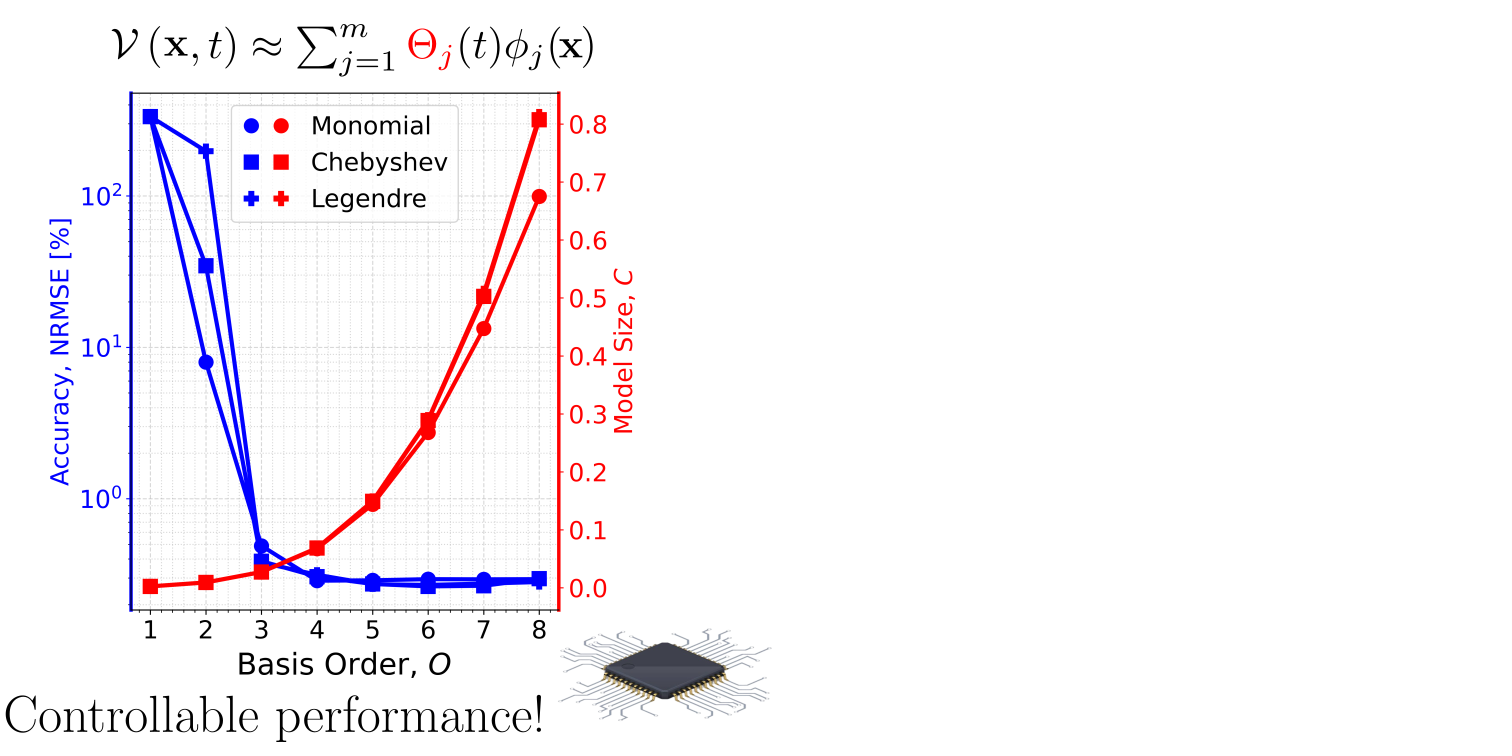
\includegraphics[width=0.9\textwidth]{../figs/sparsehjb/performance_ae_1.png}
        \end{figure}}
    \only<3>{
        \begin{figure}
            \centering
            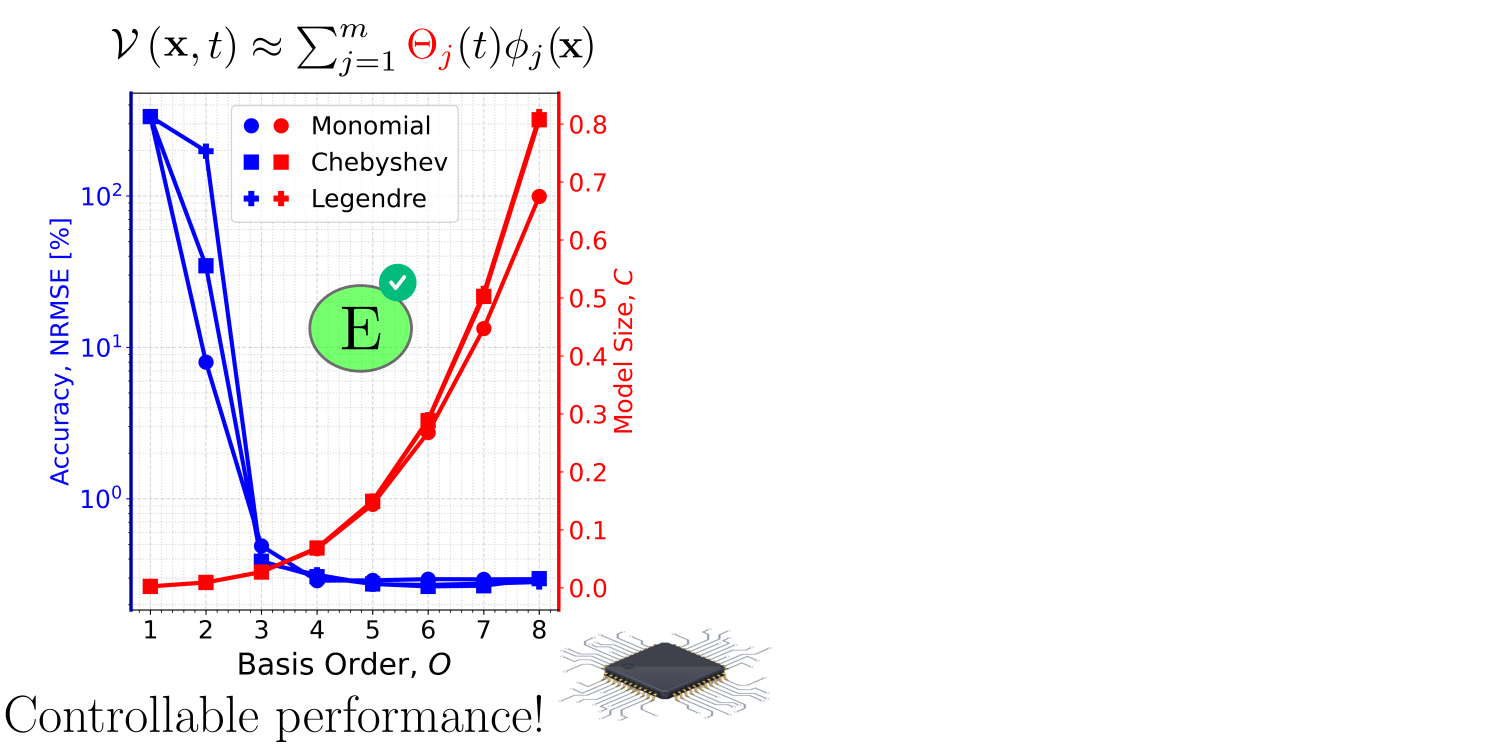
\includegraphics[width=0.9\textwidth]{../figs/sparsehjb/performance_ae_2.png}
        \end{figure}}
    \only<4>{
        \begin{figure}
            \centering
            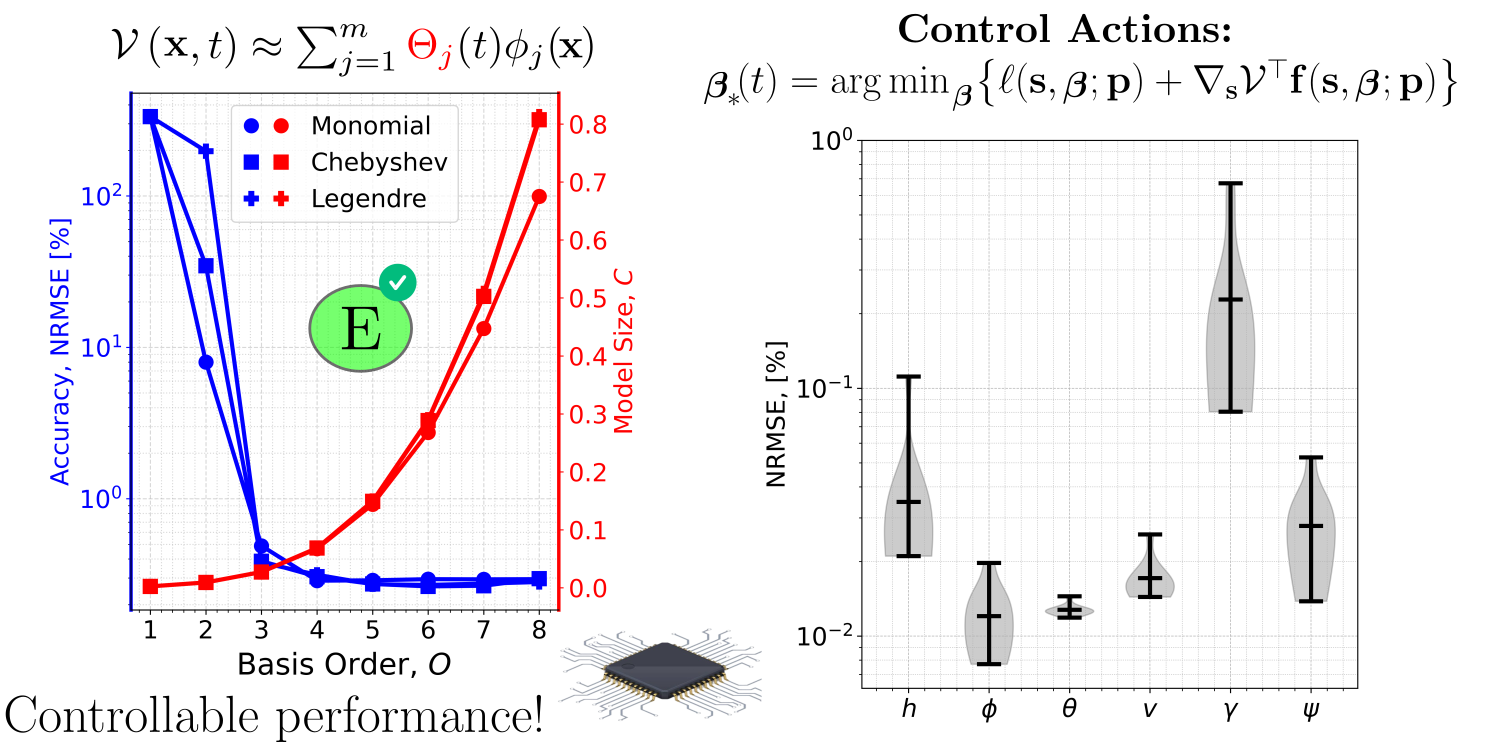
\includegraphics[width=0.9\textwidth]{../figs/sparsehjb/performance_ae_3.png}
        \end{figure}}
    \only<5>{
        \begin{figure}
            \centering
            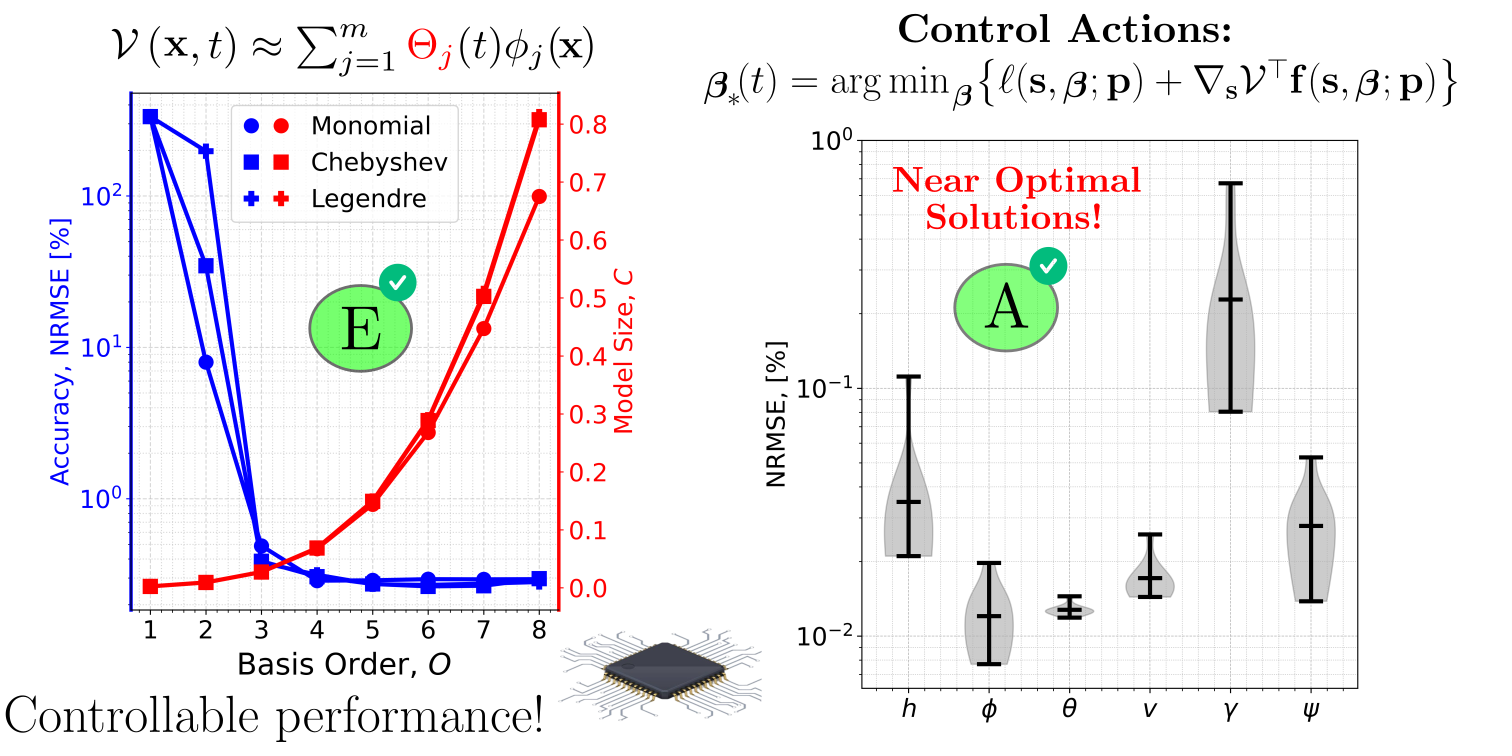
\includegraphics[width=0.9\textwidth]{../figs/sparsehjb/performance_ae_4.png}
        \end{figure}}
\end{frame}

\begin{frame}{Addressing the ITOC: Results and Analysis}
    \footnotesize
    \visible<1->{Real-time control for the \textbf{space shuttle during re-entry} to maximize \textbf{cross-range},}
    \vspace*{-0.1in}
    \begin{columns}
        \begin{column}{0.7\textwidth}
            \only<2>{
                \begin{figure}
                    \centering
                    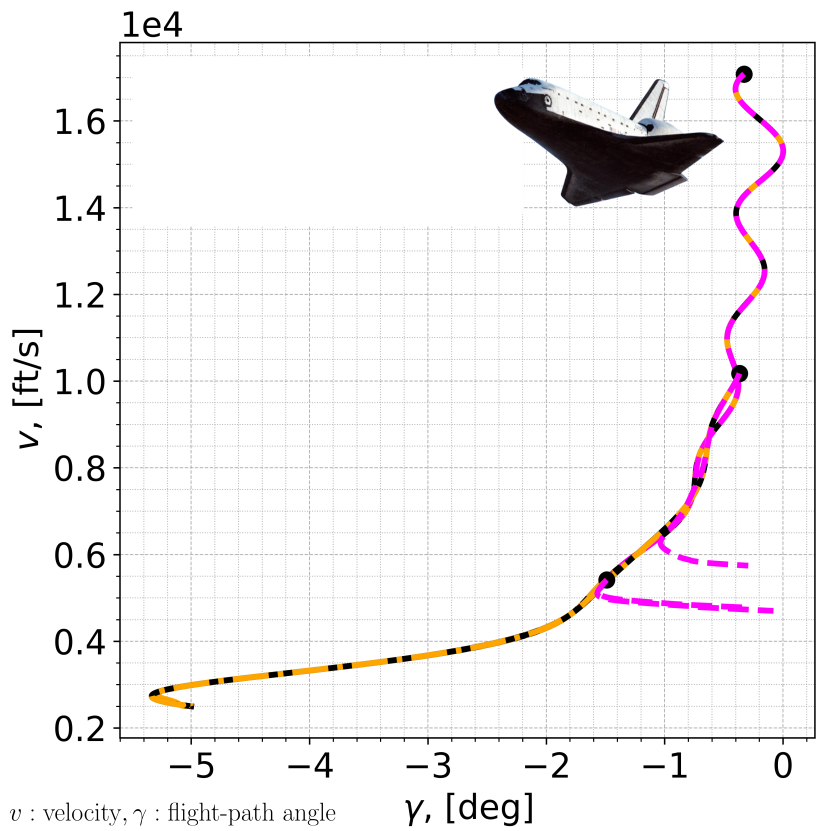
\includegraphics[width=0.65\textwidth]{../figs/sparsehjb/performance_ss_1.png}
                \end{figure}}
            \only<3>{
                \begin{figure}
                    \centering
                    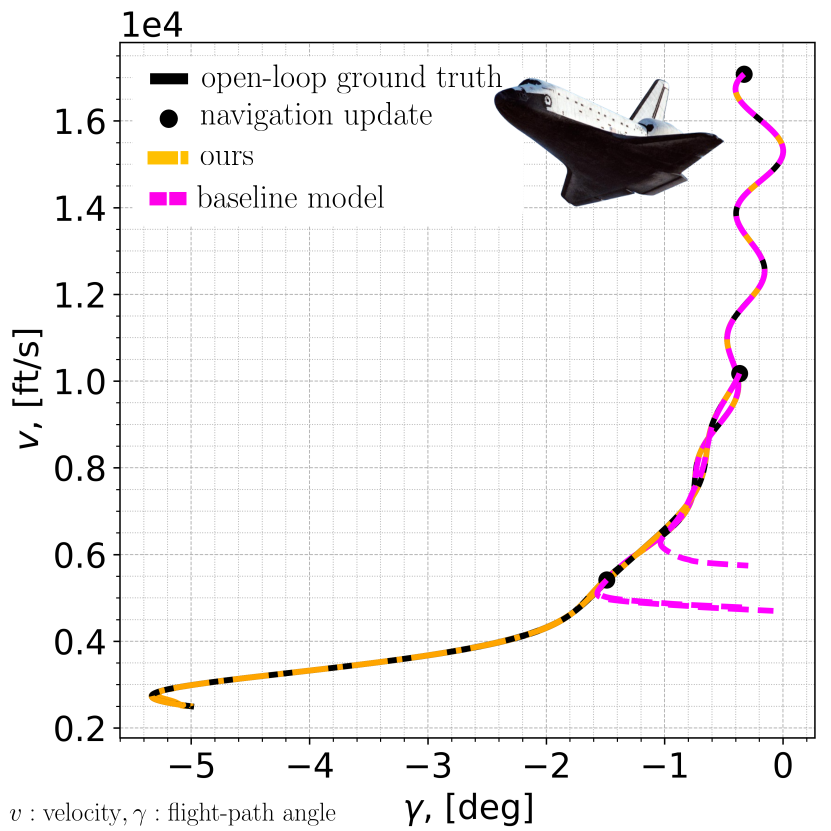
\includegraphics[width=0.65\textwidth]{../figs/sparsehjb/performance_ss_2.png}
                \end{figure}}
            \only<4>{
                \begin{figure}
                    \centering
                    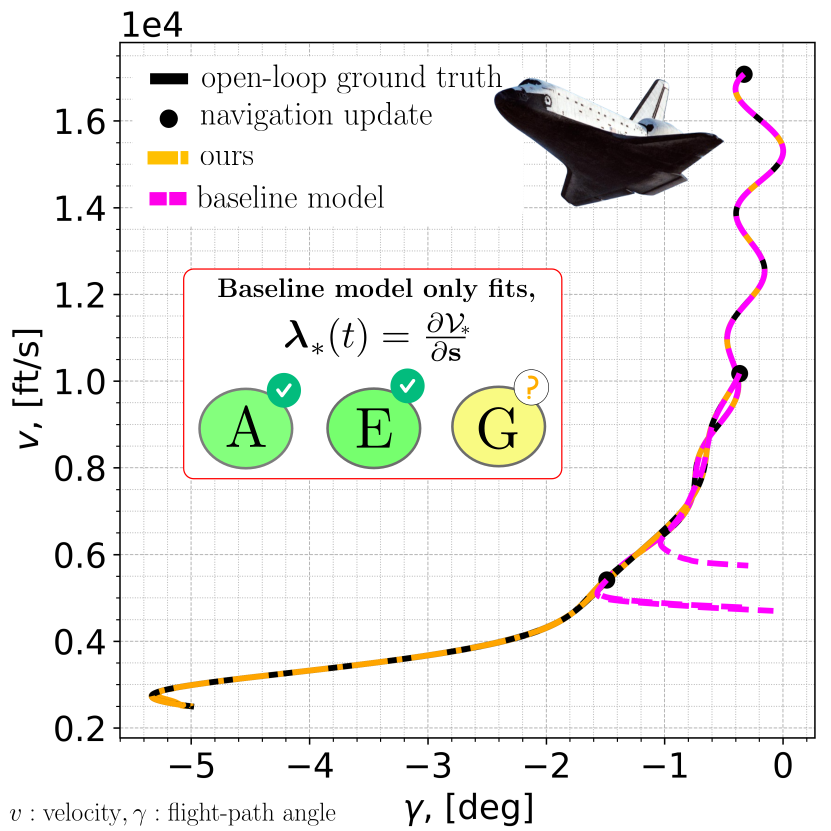
\includegraphics[width=0.65\textwidth]{../figs/sparsehjb/performance_ss_3.png}
                \end{figure}}
            \only<5->{
                \begin{figure}
                    \centering
                    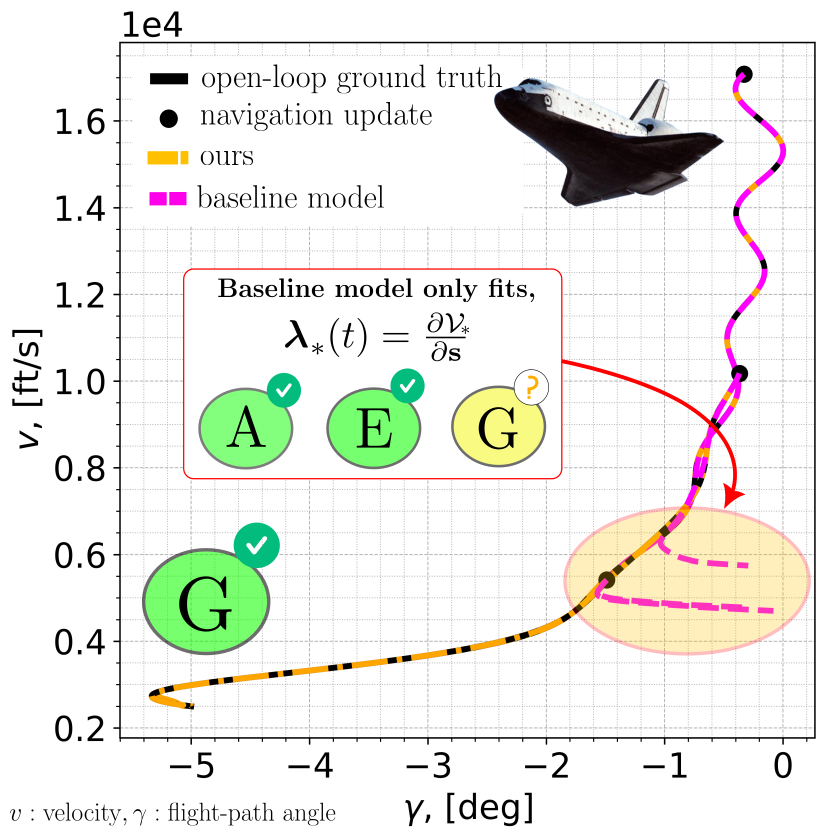
\includegraphics[width=0.65\textwidth]{../figs/sparsehjb/performance_ss_4.png}
                \end{figure}}
        \end{column}
        \hspace*{-1in}
        \begin{column}{0.4\textwidth}
            \visible<6->{
            \begin{graybox}{Key Results}
                \begin{itemize}
                    \item Improved \textbf{generalizability},
                    \vspace*{-0.05in}
                    \item \textbf{Accelerations} $\approx10^4$,
                    \vspace*{-0.05in}
                    \item \textbf{Model compressions} $\approx30\%$
                \end{itemize}
            \end{graybox}}
        \end{column}
    \end{columns}
\end{frame}

\begin{frame}{Addresing the ITOC: Results and Analysis}
    \footnotesize
    \visible<1->{Real-time control of a \textbf{hypersonic glider} to \textbf{maximize terminal velocity},}
    \vspace*{-0.1in}
    \begin{columns}
        \begin{column}{0.67\textwidth}
            \only<2>{
                \begin{figure}
                    \centering
                    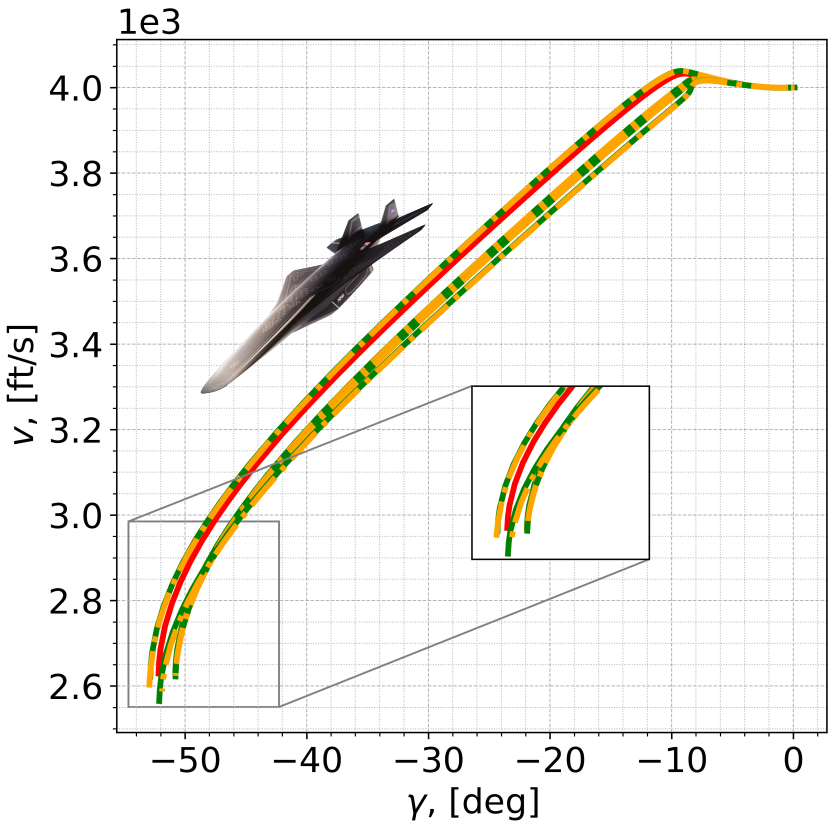
\includegraphics[width=0.65\textwidth]{../figs/sparsehjb/performance_glider_1.png}
                \end{figure}}
            \only<3>{
                \begin{figure}
                    \centering
                    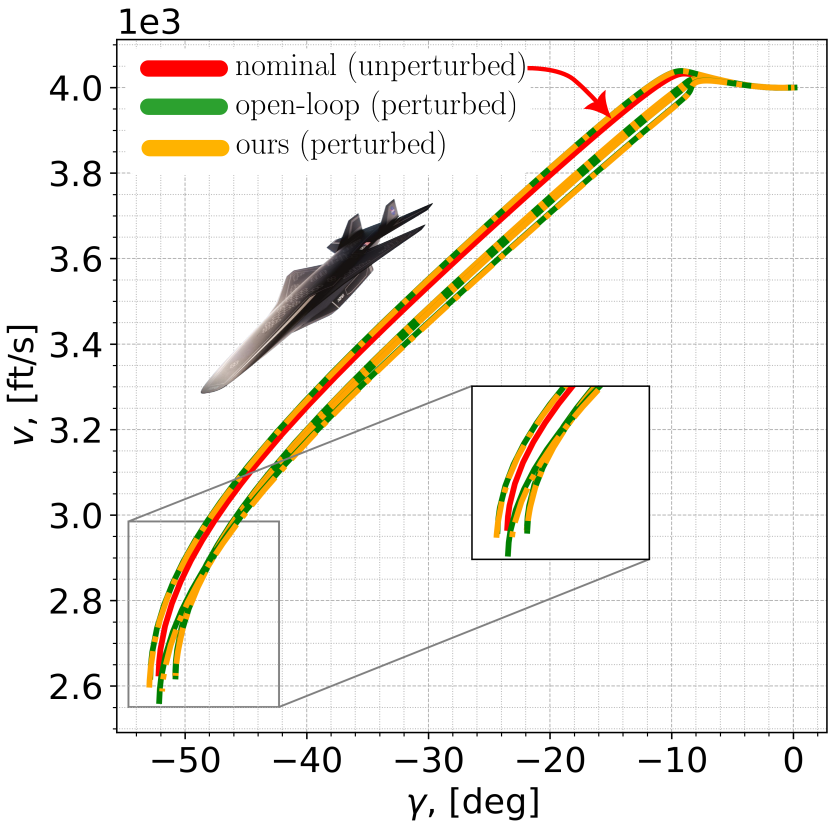
\includegraphics[width=0.65\textwidth]{../figs/sparsehjb/performance_glider_2.png}
                \end{figure}}
            \only<4>{
                \begin{figure}
                    \centering
                    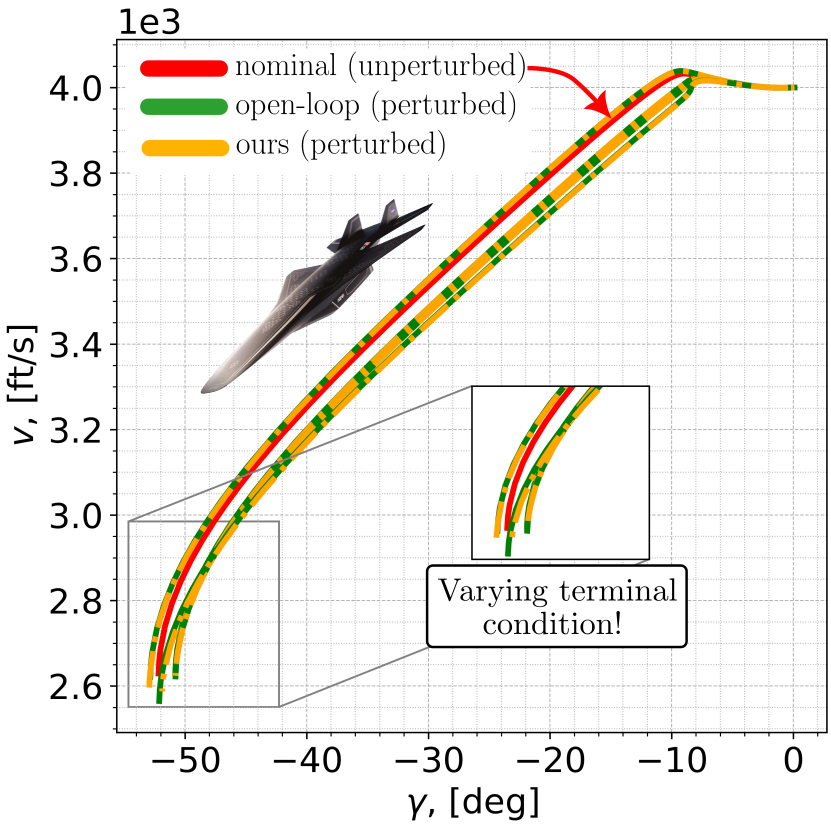
\includegraphics[width=0.65\textwidth]{../figs/sparsehjb/performance_glider_3.png}
                \end{figure}}
            \only<5>{
                \begin{figure}
                    \centering
                    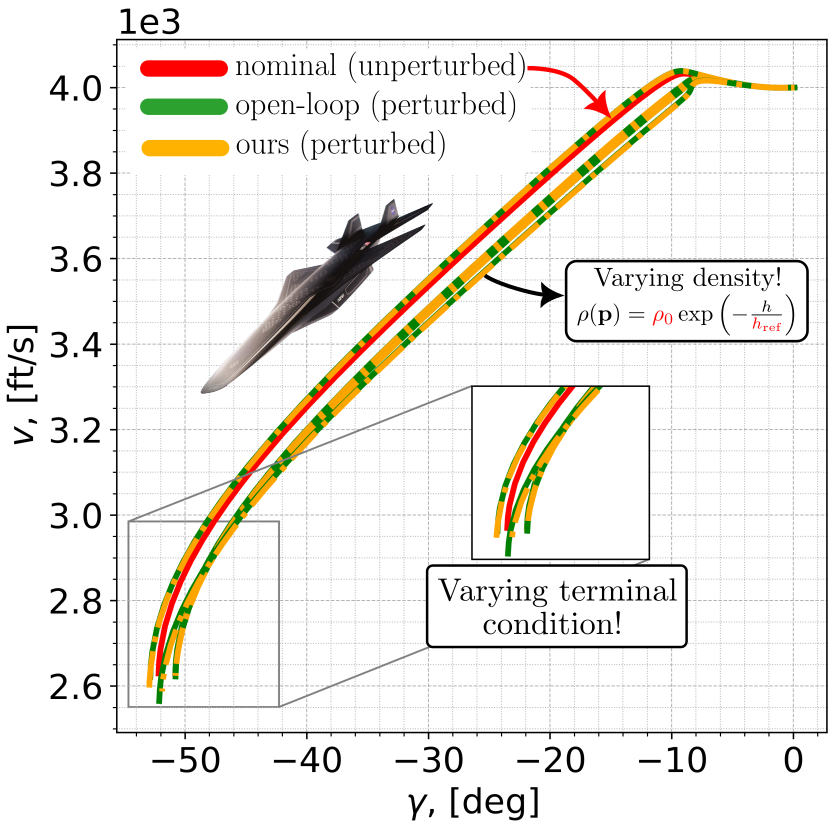
\includegraphics[width=0.65\textwidth]{../figs/sparsehjb/performance_glider_4.png}
                \end{figure}}
            \only<6->{
                \begin{figure}
                    \centering
                    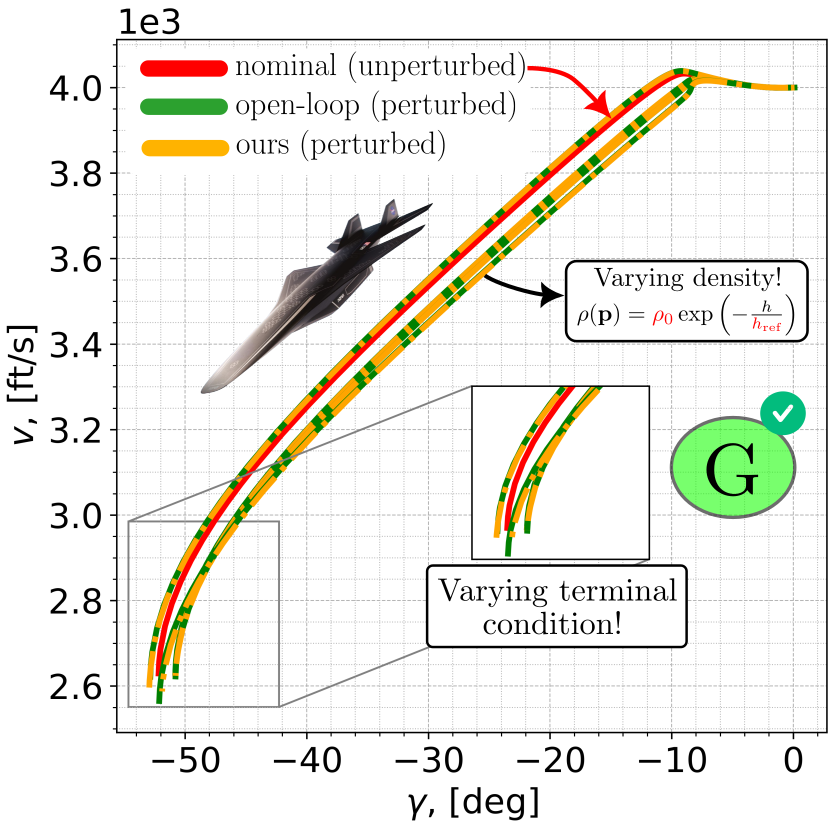
\includegraphics[width=0.65\textwidth]{../figs/sparsehjb/performance_glider_5.png}
                \end{figure}
            }
        \end{column}
        \hspace*{-1in}
        \begin{column}{0.45\textwidth}
            \visible<3->{
            \begin{graybox}{Perturbed}
                \centering
                \begin{itemize}
                    \item Varying terminal conditions,
                    \vspace*{-0.05in}
                    \item Varying atmosphere
                \end{itemize}
            \end{graybox}}
            \visible<7->{
            \begin{graybox}{Key Results}
                \begin{itemize}
                    \item Generalize to \textbf{model perturbations},
                    \vspace*{-0.05in}
                    \item \textbf{Accelerations} $\approx784$,
                    \vspace*{-0.05in}
                    \item \textbf{Model compressions} $\approx 80\%$
                \end{itemize}
            \end{graybox}}
        \end{column}
    \end{columns}
\end{frame}

\begin{frame}{Addressing the ITOC: Results and Analysis}
    \footnotesize
    \begin{columns}
        \begin{column}{0.4\textwidth}
            \centering
            \visible<1->{
            \textbf{Is the ITOC solved?}
            \begin{figure}
                \centering
                
\includegraphics[width=0.9\textwidth]{../../Chapter-1/Figures/itoc.png}
            \end{figure}}
        \end{column}
        \begin{column}{0.7\textwidth}
            \centering
            \begin{itemize}
                \item<2-> \textbf{Accuracy}: comparable to indirect OCP solutions (NRMSE $<1\%$)
                \item<3-> \colorbox{green!30}{\textbf{Efficiency}}:
                \begin{itemize}
                    \item<4-> \colorbox{green!30}{\textbf{Accelerations} $\approx 10^3 - 10^4$}
                    \item<5-> \colorbox{green!30}{\textbf{Model compressions} $\approx 80\%$}
                \end{itemize}
                \item<6-> \colorbox{green!30}{\textbf{Generalizability}: unseen BCs and model parameters}, but no guarantees outside the tube!
                \item<7-> Offline training costs \colorbox{red!30}{not quantified (future work)}
            \end{itemize}
        \end{column}
    \end{columns}
    \visible<2->{
    \begin{tikzpicture}[remember picture, overlay]
        \node[anchor=north west, xshift=2.2cm, yshift=-2.8cm] at (current page.north west) {
\includegraphics[width=0.1\textwidth]{../figs/pirom/checkmark.png}};
    \end{tikzpicture}}
    \visible<3->{
    \begin{tikzpicture}[remember picture, overlay]
        \node[anchor=north west, xshift=0.1cm, yshift=-5.8cm] at (current page.north west) {
\includegraphics[width=0.08\textwidth]{../figs/pirom/checkmark.png}};
    \end{tikzpicture}}
    \visible<5->{
    \begin{tikzpicture}[remember picture, overlay]
        \node[anchor=north west, xshift=4.45cm, yshift=-5.8cm] at (current page.north west) {
\includegraphics[width=0.1\textwidth]{../figs/pirom/checkmark.png}};
    \end{tikzpicture}}
\end{frame}